\section{Resolver el Juego Kuhn Poker}

Para resolver este juego se utilizó el procedimiento de Regret Matching con regret incondicional, el cual es el más eficiente de los $3$ procedimientos descritos. Sin embargo, para poder aplicar este algoritmo es necesario llevar el juego a su forma normal, como se describe en la sección \ref{subsec:FN-FE}. Se realizó una corrida para obtener una estrategia hasta obtener un regret menor que $5 {\times} 10^{-5}$. El tiempo total fue de $144.863$ segundos, y el número total de iteraciones fue de $4362649$. La Figura \ref{fig:regret-kuhn-poker} muestra el regret con respecto al número de iteraciones.

\begin{figure}[ht]
\caption{Gráfica del regret con respecto al número de iteraciones del juego Kuhn Poker}
\label{fig:regret-kuhn-poker}
\centering
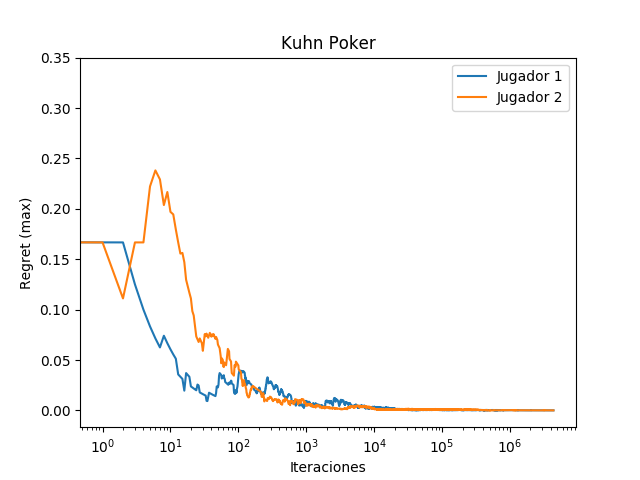
\includegraphics[width=0.4\textwidth]{graficas/kuhn-poker/grafica-kuhn-poker.png}
\end{figure}

Para mostrar la estrategia obtenida, es necesario encontrar una estrategia de comportamiento equivalente a la estrategia mixta obtenida del algoritmo de Regret Matching, como se describe en la sección \ref{subsec:EC-EM}. La Tabla \ref{tab:estrategia-kuhn-poker} muestra el equilibrio de Nash (parametrizados con el valor $\alpha$) y la estrategia obtenida del procedimiento. Se puede observar que la estrategia obtenida aproxima a un equilibrio de Nash con $\alpha \approx 0.253175$.

\begin{table}[]
    \centering
    \begin{tabular}{c|r r| r r}
        I & \multicolumn{2}{|c|}{Equilibrio de Nash} & \multicolumn{2}{|c}{Regret Matching} \\ \hline
         $1$ & $1-\alpha$ & $\alpha$ & $0.746825$ & $0.253175$ \\
         $2$ & $1$ & $0$ & $1$ & $0$ \\
         $3$ & $1$ & $0$ & $1$ & $0$ \\
         $4$ & $\frac{2}{3}$& $\frac{1}{3}$ & $0.6667$ & $0.3333$ \\
         $5$ & $0$ & $1$ & $0$ & $1$ \\
         $6$ & $1$ & $0$ & $1$ & $0$ \\
         $7$ & $0$ & $1$ & $0$ & $1$ \\
         $8$ & $\frac{2}{3}$ & $\frac{1}{3}$ & $0.6667$ & $0.3333$ \\
         $9$ & $\frac{2}{3} - \alpha$ & $\alpha + \frac{1}{3}$ & $0.412859$ & $0.587141$ \\
        $10$ & $1$ & $0$ & $1$ & $0$ \\
        $11$ & $1 - 3 \alpha$ & $3 \alpha$ & $0.240376$ & $0.759624$ \\
        $12$ & $0$ & $1$ & $0$ & $1$ \\ \hline
    \end{tabular}
    \caption{Equilibrio de Nash y estrategia obtenida para el juego de Kuhn Poker}
    \label{tab:estrategia-kuhn-poker}
\end{table}

